\chapter{Initial Value Problems and their Properties}
\label{cha:awa}
\section{Modeling with ordinary differential equations}

\begin{example}[Exponential growth]
  Bacteria are living on a substrate with ample nutrients. Each
  bacteria splits into two after a certain time $\Delta t$. The time
  span for splitting is fixed and independent of the individuum. Then,
  given the amount $u_0$ of bacteria at time $t_0$, the amount at
  $t_1 = t_0+\Delta t$ is $u_1 = 2 u_0$. Generalizing, we obtain
  \begin{gather*}
    u_n = u(t_n) = 2^n u_0, \qquad t_n = t_0 + n\Delta t.
  \end{gather*}

  After a short time, the number of bacteria will be huge, such that
  counting is not a good idea anymore. Also, the cell division does
  not run on a very sharp clock, such that after some time, divisions
  will not only take place at the discrete times $t_0+n\Delta t$, but
  at any time between these as well. Therefore, we apply the continuum
  hypothesis, that is, $u$ is not a discrete quantity anymore, but a
  continuous one that can take any real value. In order to accommodate
  for the continuum in time, we make a change of variables:
  \begin{gather*}
    u(t) = 2^{\frac{t-t_0}{\Delta t}} u_0.
  \end{gather*}

  Here, we have already written down the solution of the problem,
  which is hard to generalize. The original description of the problem
  involved the change of $u$ from one point in time to the next. In
  the continuum description, this becomes the derivative, which we can
  now compute from our last formula:
  \begin{gather*}
    \tfrac{d}{dt} u(t) = \frac{\ln 2}{\Delta t} 2^{\frac{t-t_0}{\Delta t}} u_0
    = \frac{\ln 2}{\Delta t} u(t).
  \end{gather*}
  
  We see that the derivative of $u$ at a certain time depends on $u$
  itself at the same time and a constant factor, which we call the
  growth rate $\alpha$. Thus, we have arrived at our first
  differential equation
  \begin{gather}
    \label{eq:models:1}
    u'(t) = \alpha u(t).
  \end{gather}
  What we have seen as well is, that we had to start with some
  bacteria to get the process going. Indeed, any function of the form
  \begin{gather*}
    u(t) = c e^{\alpha t}
  \end{gather*}
  is a solution to equation~\eqref{eq:models:1}. It is the initial
  value $u_0$, which anchors the solution and makes it unique.
\end{example}

\begin{example}[Predator-prey systems]
  We add a second species to our bacteria example. Let's say, we
  replace the bacteria by sardines living in a nutrient rich sea, and
  we add tuna eating sardines. The amount of sardines eaten depends on
  the likelyhood that a sardine and a tuna are in the same place, and
  on the hunting efficiency $\beta$ of the tuna. Thus,
  equation~\eqref{eq:models:1} is augmented by a negative change in
  population depending on the product of sardines $u$ and tuna $v$:
  \begin{gather*}
    u' = \alpha u - \beta u v.
  \end{gather*}

  In addition, we need an equation for the amount of tuna. In this
  simple model, we will make two assumptions: first, tuna die of
  natural causes at a death rate of $\gamma$. Second, tuna procreate
  if there is enough food (sardines), and the procreation rate is
  proportional to the amount of food. Thus, we obtain
  \begin{gather*}
    v' = \delta u v - \gamma v.
  \end{gather*}

  Again, we will need initial populations at some point in time to
  compute ahead from there.
\end{example}

\begin{remark}
  The Lotka-Volterra-equations have periodic solutions. Even though
  none of these exist in closed form the sulotions can be simulated:
  \begin{center}
  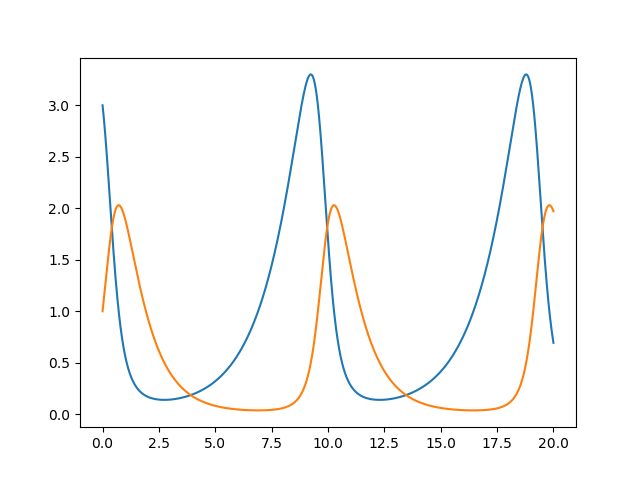
\includegraphics[width=.48\textwidth]{fig/lotkavolterra}
  \captionof{figure}{Plot of a solution to the Lotka-Volterra equation with
  parameters $\alpha = \frac 23$, $\beta  = \frac 43$, $\delta = \gamma = 1$
  and initial values $u(0) = 3$, $v(0) = 1$. Solved with a Runge-Kutta
  method of order five and step size $h = 10^{-5}$ \label{fig:lotkavolterra}}
  \end{center}
  Lotka and Volterra became interested in this system as they had
  found that the amount of predatory fish caught had increased
  during World War I. During the war years there was a strong
  decrease of fishing effort. In conclusion, they thought, there had
  to be more prey fish.
  
  A (far too rarely) applied consequence is that in order to diminish
  the amount of e.g. foxes one should hunt rabbits as foxes feed
  on rabbits.
\end{remark}

\begin{example}[Graviational two-body systems]
  According to Newton's law of universal gravitation, two bodies of
  masses $m_1$ and $m_2$ attract each other with a force
  \begin{gather*}
    \vec F_1 = G \frac{m_1m_2}{r^3} \vec r_1,
  \end{gather*}
  where $\vec F_1$ is the force vector acting on $m_1$ and $\vec r_1$
  is the vector pointing from $m_1$ to $m_2$ and $r = \lvert\vec r_1\rvert = \lvert\vec r_2\rvert$.

  Newton's second law of motion on the other hand relates forces and
  acceleration:
  \begin{gather*}
    \vec F = m \vec x'',
  \end{gather*}
  where $\vec x$ is the position of a body in space.

  Combining these, we obtain equations for the positions of the two bodies:
  \begin{gather*}
    \vec x''_i = G \frac{m_{3-i}}{r^3} (\vec x_i - \vec x_{3-i}), \qquad i=1,2.
  \end{gather*}
  This is a system of 6 independent variables. Nevertheless, it can be
  reduced to three by using that the center of mass moves
  inertially. Then, the distance vector is the only variable to be
  computed for:
  \begin{gather*}
    \vec r'' = - G \frac{m}{r^3} \vec r.
  \end{gather*}
  Intuitively, that we need an initial position and an initial
  velocity for the two bodies. Later on, we will see that this can
  actually be justified mathematically.
\end{example}

\begin{example}[Celestial mechanics]
  Now we extend the two-body system to a many-body system. Again, we
  subtract the center of mass, such that we obtain $n$ sets of 3
  equations for an $n+1$-body system. Since forces simply add up, this
  system becomes
  \begin{gather}
    \label{eq:celestial}
    \vec x_i = -G \sum_{j\neq i} \frac{m_j}{r_{ij}^3} \vec r_{ij}.
  \end{gather}
  Here, $\vec r_{ij} = \vec r_j - \vec r_i$ and $r_{ij} = \lvert \vec r_{ij}\rvert$.
  Initial data for the solar system can be obtained from
  \begin{center}
    \texttt{https://ssd.jpl.nasa.gov/?horizons}
  \end{center}
\end{example}

%%% Local Variables: 
%%% mode: latex
%%% TeX-master: "notes"
%%% End: 

%%%%%%%%%%%%%%%%%%%%%%%%%%%%%%%%%%%%%%%%%%%%%%%%%%%%%%%%%%%%%%%%%%%%%%
%%%%%%%%%%%%%%%%%%%%%%%%%%%%%%%%%%%%%%%%%%%%%%%%%%%%%%%%%%%%%%%%%%%%%%
\section{Introduction to initial value problems}
%%%%%%%%%%%%%%%%%%%%%%%%%%%%%%%%%%%%%%%%%%%%%%%%%%%%%%%%%%%%%%%%%%%%%%
%%%%%%%%%%%%%%%%%%%%%%%%%%%%%%%%%%%%%%%%%%%%%%%%%%%%%%%%%%%%%%%%%%%%%%


\begin{Definition*}{ode}{Ordinary differential equations}
  \defindex{differential equation!ordinary|see{ordinary differential equation}} \index{ODE|see{ordinary
      differential equation}} An \define{ordinary differential
    equation} (ODE) is an equation for a function $u(t)$, defined on
  an interval $I \subset \R$ and with values in the real or complex
  numbers or in the space $\R^d$ ($\C^d$), of the form
  \begin{gather}
    F\bigl(t, u(t), u'(t), u''(t), \dots, u^{(n)}(t)\bigr) = 0.
  \end{gather}
  Here $F(\ldots)$ denotes an arbitrary function of its arguments.
  The \textbf{order}\defindex{order!of a differential equation} $n$ of
  a differential equation is the highest derivative which occurs.  If
  the dimension $d$ of the value range of $u$ is higher than one, we
  talk about systems of differential equations.
\end{Definition*}

\begin{remark}
  A differential equation, which is not ordinary, is called partial.
  These are equations or systems of equations, which involve partial
  derivatives with respect to several independent variables.  While
  the functions in an ordinary differential equation may be dependent
  on additional parameters, derivatives are only taken with respect to
  one variable, typically, but not exclusively, this variable is
  time. Due to the fact that this manuscript just deals with ordinary
  differential equations, the adjective will be omitted in the
  following.
\end{remark}

\begin{Definition}{explicit-ode}{Explicit differential equation}
  \defindex{ordinary differential equation!explicit} An \define{explicit
    differential equation} of first order is a equation of the form
  \begin{align}
    \label{eq:awa:ode}
    u'(t) &= f(t,u(t))\\
    \text{or shorter:}\qquad u'&=f(t,u). \notag
  \end{align}
  A differential equation of order $n$ is called explicit, if it is of
  the form
  \begin{gather*}
    u^{(n)}(t) = F\left(t, u(t), u'(t), \ldots, u^{(n-1)}(t)\right)
  \end{gather*}
\end{Definition}
\begin{Lemma}{first-order}
  Every differential equation of higher order can be written as a
  system of first-order differential equations. If the equation is
  explicit, then the system is explicit.
\end{Lemma}

\begin{proof}
  By the introduction of additional variables $u_0(t) = u(t)$, $u_1(t)
  = u'(t)$ to $u_{n-1}(t) = u^{(n-1)}(t)$, each differential equation of
  order $n$ can be transformed into a system of $n$ differential equations
  of first order. This system has the form
  \begin{gather}
    \label{eq:awa:13}
    \begin{pmatrix}
      u_0'(t) - u_1(t) \\
      u_1'(t) - u_2(t) \\
      \vdots\\
      u_{n-2}'(t) - u_{n-1}(t) \\
      F\bigl(t, u_0(t),u_1(t),\dots,u_{n-1}(t), u_{n-1}'(t)\bigr)
    \end{pmatrix}
    =
    \begin{pmatrix}
      0\\0\\\vdots\\0\\0
    \end{pmatrix}.
  \end{gather}
  In the case of an explicit equation, the system has the form
  \begin{gather}
    \label{eq:awa:13a}
    \begin{pmatrix}
      u_0'(t) \\
      u_1'(t) \\
      \vdots\\
      u_{n-2}'(t) \\
      u_{n-1}' (t)
    \end{pmatrix}
    =
    \begin{pmatrix}
      u_1(t)\\u_2(t)\\\vdots\\u_{n-1}(t)\\F\bigl(t, u_0(t),u_1(t),\dots,u_{n-1}(t)\bigr)
    \end{pmatrix}.
  \end{gather}
\end{proof}

\begin{example}
  \label{ex:awa:sine-1}
  The differential equation
  \begin{gather}
    \label{eq:awa:17}
    u'' + \omega^2 u = f(t)
  \end{gather}
  can be transformed into the system
  \begin{gather}
    \label{eq:awa:18}
    \begin{split}
      u_1' - u_2 &= 0, \\
      u_2' + \omega^2 u_1 &= f(t).
    \end{split}
  \end{gather}
  The transformation is not uniquely determined. In this example, a
  more symmetric system can be obtained:
  \begin{gather}
    \label{eq:awa:18a}
    \begin{split}
      u_1' - \omega u_2 &= 0, \\
      u_2' + \omega u_1 &= f(t).
    \end{split}
  \end{gather}
  From a numerical perspective, system ~\ref{eq:awa:18a} should be
  chosen over ~\ref{eq:awa:18} to avoid loss of significance or overflow,
  i.e. if $|\omega| \ll 1$ or $|\omega| \gg 1$.
\end{example}

\begin{Definition}{autonomization}
  A differential equation of the form~\eqref{eq:awa:ode} is called
  \textbf{autonomous}, \defindex{autonomous differential equation} if
  the right hand side $f$ is not explicitly dependent on $t$, i.e.
  \begin{gather}
    u'=F(u).
  \end{gather}

  Each differential equation can be transformed into an autonomous
  differential equation.  This is called
  \textbf{autonomization}. \defindex{autonomization}
  \begin{equation*}
    U = \begin{pmatrix} u \\ t \end{pmatrix},
    \qquad
    F(U) = \begin{pmatrix} f(t,u) \\ 1 \end{pmatrix},
    \qquad
    U' = F(U)
  \end{equation*}

  A method which provides the same solution for the autonomous
  differential equation as for the original IVP, is called
  \textbf{invariant under autonomization}.
\end{Definition}


Differential equations usually provide sets of solutions from which we
have to choose a solution. An important selection criteria is setting
an initial value which leads to a well-posed problem (see below).

\begin{Definition}{IVP}
  \index{IVP|see{initial value problem}} Given a point
  $(t_0,u_0)\in \R \times \R^d$.  Furthermore, let the function
  $f(t,u)$ with values in $\R^d$ be defined in a neighborhood
  $I\times U \subset \R\times \R^d$ of the initial value.  Then an
  \define{initial value problem} (IVP) is defined as follows: find a
  function $u(t)$, such that
  \begin{subequations}
    \label{eq:awa}
    \begin{align}
      \label{eq:awa:2}
      u'(t)&=f\bigl(t,u(t)\bigr)
      \\
      \label{eq:awa:3}
      u(t_0)&=u_0
  \end{align}
  \end{subequations}
\end{Definition}
\begin{Definition}{local-solution}
    \label{def:awa:local solution}
  \defindex{solution!local} We call a continuously differentiable
  function $u(t)$ with $u(t_0) = 0$ a \define{local solution} of the
  IVP~\eqref{eq:awa}, if there exists a neighborhood $J$ of the point
  in time $t_0$ in which $u$ and $f(t,u(t))$ are defined and if the
  equation~\eqref{eq:awa:2} holds for all $t\in J$.
\end{Definition}

\begin{remark}
  We introduced the IVP deliberately in a ``local'' form because the
  local solution term is the most useful one for our purpose. Due to
  the fact that the neighborhood $J$ in the definition above can be
  arbitrarily small, we will have to deal with the extension to larger
  intervals below.
\end{remark}

\begin{remark}
  Through the substitution of $t\mapsto \tau$ with $\tau = t-t_0$ it
  is possible to transform every IVP at the point $t_0$ to a IVP in
  point $0$. We will make use of this fact and soon always assume
  $t_0 = 0$.
\end{remark}

\begin{Lemma}{volterra}
  Under the assumption that the right hand side $f$ is continuous in
  both arguments, the function $u(t)$ is a solution of the initial
  value problem~\eqref{eq:awa} if and only if it is a solution of the
  \define{Volterra integral equation} (VIE) \index{VIE!see{Volterra
      integral equation}}
  \begin{gather}
    \label{eq:volterra}
    u(t) = u_0 + \int_{t_0}^t f\bigl(s,u(s)\bigr)\ds.
  \end{gather}
  The formulation as integral equation allows on the other hand a more
  general solution term, because the problem is already well-posed for
  functions $f(t,u)$, which are just integrable with respect to $t$.
  In that case the solution $u$ would be just absolutely continuous
  and not continuously differentiable.
\end{Lemma}

%%% Local Variables: 
%%% mode: latex
%%% TeX-master: "../notes"
%%% End: 


\begin{remark}
  Both the theoretical analysis of the IVP and the numerical methods
  (with exception of the BDF methods) in this lecture notes, solve
  actually never the IVP~\eqref{eq:awa} but always the associated
  integral equation ~\eqref{eq:volterra}.
\end{remark}

\begin{Theorem*}{peano}{Peano's existence theorem}
  \defindex{Peano's theorem}
  \label{satz:peano}
  Let the function $f(t,u)$ be continuous on the closed set
  \begin{gather*}
    \overline D =\bigl\{
    (t,u) \in \R\times\R^d \;\big|
    \;|t-t_0| \le \alpha,\;
    |u-u_0|\le\beta
    \bigr\},
  \end{gather*}
  where $\alpha,\beta>0$. Then there exists a solution
    $u(t) \in C^1(I)$
  on the interval
    $I=[t_0-T,t_0+T]$
  with
  \begin{gather*}
    T=\min\left(\alpha ,\frac{\beta}{M}\right),\;
    M=\max_{(t,u)\in \overline D} \ |f(t,u)|.
  \end{gather*}
\end{Theorem*}


The proof of this theorem is of little consequence for the remainder
of these notes.  For its verification, we refer to textbooks on the
theory of ordinary differential equations.

\begin{remark}
  The Peano existence theorem does not make any statements about the
  uniqueness of a solution and also just guarantees local existence.
  The second limitation is addressed by the following theorem. The
  first will be postponed to section~\ref{sec:awa:well-posedness}.
\end{remark}

\begin{Theorem*}{peano-continuation}{Peano's continuation theorem}
  Let the assumptions of Theorem~\ref{satz:peano} hold. Then, the
  solution can be extended to an interval $I_m = [t_-, t_+]$ such that
  the points $\bigl(t_-,u(t_-)\bigr)$ and $\bigl(t_+,u(t_+)\bigr)$ are
  on the boundary of $\overline D$. Neither the values of $t$, nor of
  $u(t)$ need to be bounded as long as $f$ remains bounded.
\end{Theorem*}

\begin{example}
  The IVP
  \begin{gather*}
    u' = 2 \sqrt{\lvert u \rvert}, \qquad u(0) = 0,
  \end{gather*}
  has solutions $u(t) = t^2$ and $u(t) = 0$.
\end{example}

\begin{example}
  The functions $1/(t-t_0)$ are solutions to the IVP
  \begin{gather*}
    u'=-u^2, \qquad u(t_0) = 1.
  \end{gather*}
\end{example}

%%%%%%%%%%%%%%%%%%%%%%%%%%%%%%%%%%%%%%%%%%%%%%%%%%%%%%%%%%%%%%%%%%%%%%
%%%%%%%%%%%%%%%%%%%%%%%%%%%%%%%%%%%%%%%%%%%%%%%%%%%%%%%%%%%%%%%%%%%%%%
\section{Linear differential equations
  and Grönwall's inequality}
%%%%%%%%%%%%%%%%%%%%%%%%%%%%%%%%%%%%%%%%%%%%%%%%%%%%%%%%%%%%%%%%%%%%%%
%%%%%%%%%%%%%%%%%%%%%%%%%%%%%%%%%%%%%%%%%%%%%%%%%%%%%%%%%%%%%%%%%%%%%%

\begin{intro}
  The examination of linear differential equation turns out to be
  particularly simple. On the other hand, results obtained here will
  provide us with important statements for general non-linear
  IVP. Therefore we pay particular attention to the linear case.
\end{intro}

\begin{Definition}{linear-ode}
    \defindex{ordinary differential equation!linear} An IVP according to
  definition ~\ref{Definition:IVP} is called \textbf{linear} \defindex{linear
    differential equation} if the right hand side $f$ is an affine
  function of $u$. Thus, we can write it in the form
  \begin{subequations}    
    \label{eq:awa:4}
    \begin{xalignat}{2}
      \label{eq:awa:5}
      u'(t) &= A(t)u(t) + b(t)
      & \forall t &\in \R \\
      \label{eq:awa:6}
      u(t_0) &= u_0
    \end{xalignat}
  \end{subequations}
  with a continuous matrix function $A:\R\to \C^{d \times d}$. If in
  addition $b(t) \equiv 0$, we call it \define{homogeneous}.
\end{Definition}
\begin{Definition}{integrating factor}
    Let be the matrix function $A:I\to \C^{d\times d}$ continuous.  Then
  the function defined by
  \begin{gather}
    \label{eq:awa:7}
    M(t) = \exp\left(-\int_{t_0}^t A(s) \ds\right)
  \end{gather}
  is called \define{integrating factor} of the
  equation~\eqref{eq:awa:5}.
\end{Definition}

\begin{corollary}
  The integrating factor $M(t)$ has the properties
  \begin{align}
    \label{eq:awa:14}
    M(t_0) &= \identity\\
    \label{eq:awa:15}
    M'(t) &= -M(t)A(t).
  \end{align}
\end{corollary}

\begin{Lemma}{linear-representation}
  % Voraussetzungen an A und b
  A solution of the IVP~\eqref{eq:awa:4} is given through the 
  representation
  \begin{gather}
    \label{eq:awa:8}
    u(t) =  M(t)^{-1}\left(u_0 + \int_{t_0}^t M(s) b(s) \ds\right)
  \end{gather}
  with the integrating factor $M(t)$ of the equation~\eqref{eq:awa:7}.
  This solution exists for all $t\in \R$.
\end{Lemma}


%%% Local Variables:
%%% mode: latex
%%% TeX-master: "../notes"
%%% End:


\begin{proof}
  We consider the auxiliary function $w(t) = M(t) u(t)$ with the
  integrating factor $M(t)$ of the equation~\eqref{eq:awa:7}. Using the
  product rule, there holds
  \begin{gather}
    \label{eq:awa:19}
    w'(t) =  M(t) u'(t) + M'(t) u(t)
    =  M(t) u'(t) - M(t)A(t)u(t).
  \end{gather}
  Comparing this to the differential equation~\eqref{eq:awa:5}, we see
  that $w$ solves
  \begin{gather*}
    w'(t) = M(t) b(t).
  \end{gather*}
	This can be integrated directly to obtain	
  \begin{gather*}
    w(t) = u_0 + \int_{t_0}^t M(s) b(s) \ds,
  \end{gather*}
  where we use that $w(t_0) = u_0$.  According to
  lemma~\ref{Lemma:appendix:exp-1} about the \putindex{matrix
    exponential}, $M(t)$ is invertible for all $t$.  With the
  definition of $w(t)$ we are therefore able to solve for $u(t)$,
  which results in the equation~\eqref{eq:awa:8}. The global
  solvability follows from the fact that the solution is defined for
  arbitrary $t\in \R$.
\end{proof}

\begin{example}
  \label{ex:awa:sine-2}
  The equation in example~\ref{ex:awa:sine-1} is linear and can be
  written in the form of~\eqref{eq:awa:4} with
  \begin{align*}
    A(t) = A &=
    \begin{pmatrix}
      0 & \omega \\ -\omega & 0
    \end{pmatrix}
    \\
    b(t) &= f(t).
  \end{align*}
  Let now $f(t) \equiv 0$. The Jordan canonical form of $A$ is
  \begin{gather*}
    A = C^{-1}
    \begin{pmatrix}
      \omega i \\ & -\omega i
    \end{pmatrix}
    C
  \end{gather*}
  with a suitable transformation matrix $C$. The integrating factor is
  \begin{gather*}
    M(t) = e^{At} = C^{-1}
    \begin{pmatrix}
      e^{\omega i} \\ & e^{-\omega i}
    \end{pmatrix} C
    =
    \begin{pmatrix}
      \cos \omega t & \sin \omega t \\
      -\sin \omega t & \cos \omega t
    \end{pmatrix}.
  \end{gather*}
  Thus, given an initial value $(u_0, v_0)^T$, the solution is
  \begin{gather*}
    u(t) =  \begin{pmatrix}
      \cos \omega t & \sin \omega t \\
      -\sin \omega t & \cos \omega t
    \end{pmatrix}
    \begin{pmatrix}
      u_0\\v_0
    \end{pmatrix}.
  \end{gather*}
  The missing details in this argument and the case for an
  inhomogenety $f(t) = \cos \alpha t$ are left as an exercise.
\end{example}

\begin{remark}
  If the function $b(t)$ in~\eqref{eq:awa:5} is only integrable, the
  function $u(t)$ defined in~\eqref{eq:awa:8} is absolutely continuous
  and thus differentiable almost everywhere. The chain
  rule~\eqref{eq:awa:19} is applicable in all points of
  differentiability and $w(t)$ solves the Volterra integral equation
  corresponding to~\eqref{eq:awa:4}. Thus, the representation
  formula~\eqref{eq:awa:8} holds generally for solutions of linear
  Volterra integral equations.
\end{remark}

%%%%%%%%%%%%%%%%%%%%%%%%%%%%%%%%%%%%%%%%%%%%%%%%%%%%%%%%%%%%%%%%%%%%%%
\begin{Lemma*}{gronwall}{Grönwall}
  Let be $w(t)$, $a(t)$ and $b(t)$ be nonnegative, integrable
  functions, such that $a(t)w(t)$ is integrable. Furthermore, let
  $b(t)$ be monotonically nondecreasing and let $w(t)$ satisfy the
  integral inequality
  \begin{gather}
    \label{eq:awa:10}
    w(t) \le b(t) + \int_{t_0}^t a(s)w(s)\ds,\qquad t\ge t_.
  \end{gather}
  Then, for almost all $t \ge t_0$ there holds:
  \begin{gather}
    \label{eq:awa:11}
    w(t) \le b(t) \exp\left( \int_{t_0}^t  a(s) \ds\right).
  \end{gather}
\end{Lemma*}

%%% Local Variables:
%%% mode: latex
%%% TeX-master: "../notes"
%%% End:

\begin{proof}
  Using the integrating factor
  \begin{gather*}
    m(t) = \exp\left(-\int_{t_0}^t a(s) \ds\right),
    \quad
    \frac1{m(t)} = \exp\left(\int_{t_0}^t a(s) \ds\right),
  \end{gather*}
  we introduce the auxiliary function
  \begin{gather*}
    v(t) = m(t) % \exp\left(-\int_{t_0}^t a(s) \ds\right)
    \int_{t_0}^t a(s)w(s)\ds,
  \end{gather*}
  This function is absolutely continuous and almost everywhere
  \begin{gather*}
    v'(t) = m(t) a(t) %\exp\left(-\int_{t_0}^t a(s) \ds\right)
    \left[
      w(t) - \int_{t_0}^t a(s) w(s) \ds
    \right].
  \end{gather*}
  By assumption~\eqref{eq:awa:10}, the bracket on the right is bounded
  by $b(t)$. Thus,
  \begin{gather*}
    v'(t) \le m(t) a(t) b(t) %\exp\left(-\int_{t_0}^t a(s) \ds\right),
  \end{gather*}
  and since $v(t_0) = 0$ by its definition,
  \begin{gather*}
    v(t) \le \int_{t_0}^t m(s) a(s) b(s) % \exp\left(-\int_{t_0}^s a(r)
    \ds.
  \end{gather*}
  From the definition of $v(t)$, we obtain
  \begin{gather*}
    \int_{t_0}^t a(s)w(s)\ds = \frac1{m(t)} % \exp\left(\int_{t_0}^t a(s) \ds\right)
    v(t)
    \le \frac1{m(t)} \int_{t_0}^t m(s)a(s)b(s) \ds
    % \exp\left( %\int_{t_0}^t a(r) \dr
    %   - \int_{t_0}^s a(r) \dr\right)\ds
  \end{gather*}
  Finally, since $b(t)$ is nondecreasing we obtain almost everywhere
  \begin{align*}
    \int_{t_0}^t a(s)w(s)\ds
    &\le  \frac{b(t)}{m(t)} \int_{t_0}^t a(s)
    \exp\left(-\int_{t_0}^s a(r) \dr\right)\ds
    \\
    &= \frac{b(t)}{m(t)} \left[-
    \exp\left(-\int_{t_0}^s a(r) \dr\right)
      \right]_{t_0}^t
    \\
    &= \frac{b(t)}{m(t)} \bigl(m(t_0)-m(t)\bigr)
      = \frac{b(t)}{m(t)} - b(t)
  \end{align*}
  Now, entering into the integral inequality~\eqref{eq:awa:10}, we
  obtain
  \begin{gather*}
    w(t) \le b(t) + \int_{t_0}^t a(s)w(s)\ds = \frac{b(t)}{m(t)},
  \end{gather*}
  which proves the lemma.
\end{proof}

%%%%%%%%%%%%%%%%%%%%%%%%%%%%%%%%%%%%%%%%%%%%%%%%%%%%%%%%%%%%%%%%%%%%%%

\begin{remark}
	On the form of the requirements~\eqref{eq:awa:10} as well as the
  estimation~\eqref{eq:awa:11}, we can see that Grönwall's
  inequality is basically based on the construction of a majorant for 
	$w(t)$, which satisfies a linear IVP.
\end{remark}

%%%%%%%%%%%%%%%%%%%%%%%%%%%%%%%%%%%%%%%%%%%%%%%%%%%%%%%%%%%%%%%%%%%%%%
\begin{Corollary}{awa:unique-linear}
  Let the functions $u(t)$ and $v(t)$ be two solutions of the linear
  differential equation~\eqref{eq:awa:5}. If both functions
  coincide in a point $t_0$ then they are identical.
\end{Corollary}

\begin{proof}
	The difference $w(t) = v(t) - u(t)$ solves the integral equation
  \begin{gather*}
    w(t) = \int_{t_0}^t A(s) w(s) \ds.
  \end{gather*}
  Hence $|w(t)|$ satisfies the integral inequality
  \begin{gather*}
    |w(t)| \le \int_{t_0}^t |A(s)| |w(s)| \ds,
  \end{gather*}
	from which we conclude with Grönwall's inequality~\eqref{eq:awa:11} 
	for $b(t) = 0$, that $|w(t)|=0$ for all $t$ and therefore
  $u(t) = v(t)$.
\end{proof}

\begin{corollary}
  The representation formula~\eqref{eq:awa:8} in
  Lemma~\ref{Lemma:linear-representation} defines the unique solution to the
  IVP~\eqref{eq:awa:4}. In particular, solutions of linear IVP are
  always defined on the whole real axis.
\end{corollary}

\begin{example}
  Let $A \in \C^{d\times d}$ be diagonalizable with possibly repeated
  eigenvalues $\lambda_1,\dots,\lambda_d$ and corresponding
  eigenvectors $\psi^{(i)}$. Let $\Psi$ be the matrix of column
  vectors $\psi^{(i)}$. Then, the solution of the IVP
  \begin{gather*}
    \begin{split}
      u' &= A u,\\
      u(0) &= u_0,
    \end{split}
  \end{gather*}
  is given by the formula
  \begin{gather*}
    u(t) = e^{At} u_0 = \Psi \exp
    \begin{pmatrix}
      \lambda_1\\&\ddots\\&&\lambda_d
    \end{pmatrix}
    \Psi^{-1} u_0.
  \end{gather*}
  This is due to the fact, that $M(t) = e^{-At}$ and $e^{-\Psi A
    \psi^{-1}t} = \Psi e^{-At} \Psi^{-1}$.
\end{example}
%%%%%%%%%%%%%%%%%%%%%%%%%%%%%%%%%%%%%%%%%%%%%%%%%%%%%%%%%%%%%%%%%%%%%%

\begin{Lemma}{solution-space}
  \index{homogeneous}
  \index{ordinary differential equation!linear!homogeneous}
  The solutions of the homogeneous, linear differential equation
  \begin{gather}
    \label{eq:awa:9}
    u'(t) = A(t) u(t)
  \end{gather}
  with $u:\R\to\R^d$, define a vector space of dimension $d$. Let
  $\{\psi^{(i)}\}_{i=1,\dots,d}$ be a basis of $\R^d$. 
	Then the solutions $\phi^{(i)}(t)$ of the equation~\eqref{eq:awa:9} with 
  initial values $\phi^{(i)}(0) = \psi^{(i)}$ form a basis of the solution
  space. The vectors $\{\phi^{(i)}(t)\}$ are linear independent
  for all $t\in \R$.
\end{Lemma}


\begin{proof}
  At first we observe that for two solutions $u(t)$ and $v(t)$ of the
  equation~\eqref{eq:awa:9}, their sum and their scalar multiples are
  solutions too, due to linearity \index{linear} of the derivative
  and the right hand side.  Therefore the vector space structure is
  proven.
 
  Let now $\phi^{(i)}(t)$ be solutions of the IVP with linear
  independent initial values $\{\psi^{(i)}\}$.  As a consequence the
  functions are linear independent as well.

  Assume that $w(t)$ is a solution of the equation~\eqref{eq:awa:9},
  which cannot be written as a linear combination of $\psi^{(i)}$.
  Then $w(0)$ is not a linear combination of the vectors $\psi^{(i)}$:
  else let's say $w(0) = \sum \alpha_i \psi^{(i)}$, then
  $w(t) = \sum \alpha_i \phi^{(i)}(t)$ would be a linear combination
  because of uniqueness proven in
  corollary~\ref{Corollary:awa:unique-linear}.  Since $\{\psi^{(i)}\}$
  according to the assumtions is a basis of $\R^d$, such a $w(0)$
  cannot exist.  Hence it is shown that $\phi^{(i)}(t)$ is a basis of
  the solution space of dimension $d$.
  
  It remains to show that the $\phi^{(i)}(t)$ are linearly independent
  for all $t\in \R$. To this end, assume that the set $\phi^{(i)}(t)$
  is linearly dependent for a value $t_1$.  Then the following holds
  true without loss of generality
  \begin{gather*}
    \phi^{(d)}(t_1) = \sum_{i=1}^{d-1}\alpha_i\phi^{(i)}(t_1) =: w(t).
  \end{gather*}
  Again according to corollary~\ref{Corollary:awa:unique-linear} we
  have $\phi^{(d)} \equiv w$, moreover $\phi^{(d)}(0) = w(0)$ which
  again is a contradiction to the assumption $\psi^{(d)}$ is a linear
  combination of the other initial values.
\end{proof}

%%%%%%%%%%%%%%%%%%%%%%%%%%%%%%%%%%%%%%%%%%%%%%%%%%%%%%%%%%%%%%%%%%%%%%

\begin{Definition}{fundamental-system}
  A basis $\{\phi^{(1)},\dots,\phi^{(d)}\}$ of the solution space of
  the linear differential equation~\eqref{eq:awa:9}, in particular the
  basis with initial values $\phi^{(i)}(0) = e_i$, is called
  \define{fundamental system} of solutions.  The
  matrix function
  \begin{gather}
    \label{eq:awa:12}
    \fundam(t) =
    \begin{pmatrix}
      \phi^{(1)}(t)\dots\phi^{(d)}(t)
    \end{pmatrix}
  \end{gather}
  with column vectors $\phi^{(i)}(t)$ is called
  \define{fundamental matrix}.
\end{Definition}



\begin{Corollary}{fundamental-regular}
  The fundamental matrix is regular for all $t\in \R$ and solves the
  IVP
  \begin{align*}
    \fundam'(t) &= A(t)\fundam(t)\\
    \fundam (0) &= \identity.
  \end{align*}
\end{Corollary}

\begin{proof}
  The initial value is part of the definition. On the other hand,
  splitting the the matrix valued IVP into its column vectors, we
  obtain the original IVP defining the solution space. Regularity
  follows from linear independence of solutions for any $t$.
\end{proof}

%%%%%%%%%%%%%%%%%%%%%%%%%%%%%%%%%%%%%%%%%%%%%%%%%%%%%%%%%%%%%%%%%%%%%%
%%%%%%%%%%%%%%%%%%%%%%%%%%%%%%%%%%%%%%%%%%%%%%%%%%%%%%%%%%%%%%%%%%%%%%
\section{Well-posedness of the IVP}
%%%%%%%%%%%%%%%%%%%%%%%%%%%%%%%%%%%%%%%%%%%%%%%%%%%%%%%%%%%%%%%%%%%%%%
%%%%%%%%%%%%%%%%%%%%%%%%%%%%%%%%%%%%%%%%%%%%%%%%%%%%%%%%%%%%%%%%%%%%%%
\label{sec:awa:well-posedness}


\begin{Definition}{hadamard} 
  A mathematical problem is called \define{well-posed} if the
  following \textbf{Hadamard conditions} are satisfied:
  \index{Hadamard conditions}
  \begin{enumerate}
  \item A solution exists.
  \item The solution is unique.
  \item The solution is continuously dependent on the data.
  \end{enumerate}
  The third condition in this form is purely qualitative. Typically,
  in order to characterize problems with good approximation
  properties, we will require \putindex{Lipschitz continuity}, which
  has a more quantitative character.
\end{Definition}

%%% Local Variables:
%%% mode: latex
%%% TeX-master: "../notes"
%%% End:


\begin{example}
  The IVP
  \begin{gather*}
    u'= \sqrt[3]{u}, \qquad u(0) = 0,
  \end{gather*}
  has solutions of the form
  \begin{gather*}
    u(t) =
    \begin{cases}
      0 \\
      c \left(\tfrac23t\right)^{3/2}.
    \end{cases}
  \end{gather*}
  Thus, the solution is not unique and therefore, the IVP is not
  well-posed.
  Let now the initial value be nonzero, but slightly positive. Then, a small
  perturbation, which changes its sign, will have dramatic effect on
  the solution.
\end{example}

\begin{Definition}{Lipschitz-condition}
  The function $f(t,y)$ satisfies on its domain $D = I\times\Omega \subset
  \R \times \R^d$ an uniformly continuous \define{Lipschitz condition} if 
	it is Lipschitz continuous with regard to $y$, i.e., it exists a 
	positive constant $L$, such that
  \begin{gather}
    \label{eq:awa:1}
    \forall t\in I;\,x,y\in\Omega \;:\;
    \abs{f(t,x)-f(t,y)} \le L \abs{x-y}
  \end{gather}
  It satisfies a local Lipschitz condition if the same holds true for all 
  compact subsets of $D$.
\end{Definition}


\begin{example}
  Let $f(t,u)\in C^1(\R \times\R^d )$ and let all partial derivatives
  with respect to components of $u$ be bounded by
  \begin{gather*}
    \max_{\substack{t\in \R\\u\in \R^d\\1\le i,j \le d}}
   \abs{
     \frac{\partial}{\partial u_i} f_j(t,u)
   } \le K.
  \end{gather*}
  Then, $f$ satisfies the Lipschitz condition~\eqref{eq:awa:1} with
  $L=K$. Indeed, by using Taylor expansion, we see that
  \begin{multline*}
    f_j(t, u) - f_j(t,v)
    = \int_0^1 \frac{d}{ds}f_j\bigl(t,u+s(v-u)\bigr)\ds\\
    = \int_0^1 \sum_{i=1}^d(u_i-v_i)\partial_if_j\bigl(t,u+s(v-u)\bigr)\ds.
  \end{multline*}
  It is an easy conclusion that
  \begin{gather*}
    \abs{f(t,u)-f(t,v)}
    \le K \abs{u-v}.
  \end{gather*}
\end{example}


\begin{Theorem*}{awa-stability}{Stability}
  Let $f(t,u)$ and $g(t,u)$ be two continuous functions on a
  cylinder $D = I \times \Omega$ where the interval $I$ contains
  $t_0$ and $\Omega$ is a convex set in $\R^d$.  Furthermore, let
  $f$ admit a Lipschitz condition with constant $L$ on $D$. Let $u$
  and $v$ be solutions to the IVP
  \begin{xalignat}{2}
    \label{eq:awa:20}
    u'&=f(t,u) \quad\forall t\in I,& u(t_0)&= u_0,\\
    \label{eq:awa:21}
    v'&=g(t,v) \quad\forall t\in I,& v(t_0)&= v_0.
  \end{xalignat}
  Then, there holds
  \begin{gather}
    \label{eq:awa:22}
    \abs{u(t)-v(t)} \le e^{L|t-t_0|}
    \left[ \abs{u_0-v_0}
      + \int_{t_0}^{t} \max_{x\in\Omega}
      \abs{f(s,x)-g(s,x)}\ds
    \right].
  \end{gather}
\end{Theorem*}

%%% Local Variables:
%%% mode: latex
%%% TeX-master: "../notes"
%%% End:


\begin{proof}
  Both $u(t)$ and $v(t)$ solve their respective Volterra integral
  equations. Taking the difference, we obtain
  \begin{align*}
    u(t)-v(t) &= u_0-v_0
           + \int_{t_0}^t \bigl[ f(s,u(s)) - g(s,v(s)) \bigr]\ds
    \\
         &= u_0-v_0
           + \int_{t_0}^t \bigl[ f(s,u(t)) - f(s,v(s)) \bigr]\ds
           + \int_{t_0}^t \bigl[ f(s,v(t)) - g(s,v(s)) \bigr]\ds.
  \end{align*}
  Thus, its norm admits the integral inequality
  \begin{align*}
    \abs{u(t)-v(t)}
    &\le \abs{u_0-v_0} + \int_{t_0}^t\abs{f(s,u(t)) - f(s,v(s))} \ds
    + \int_{t_0}^t \abs{f(s,v(t)) - g(s,v(s))} \ds
    \\
    &\le \underbrace{\abs{u_0-v_0}
      + \int_{t_0}^t \max_{x\in\Omega} \abs{f(s,x)-g(s,x)}\ds}_{b(t)}
      + \int_{t_0}^t L \abs{u(s)-v(s)} \ds.
  \end{align*}
  This inequality is in the form of the assumption in Grönwall's
  lemma, and its application yields the stability result.
\end{proof}


\begin{Theorem*}{picardlindelof}{Picard-Lindelöf}
  \defindex{Picard-Lindelöf theorem} 
  Let $f(t,y)$ be continuous on a cylinder
  \begin{gather*}
    D = \{ (t,y) \in \R \times
    \R^d | \ |t-t_0| \le a, |y-u_0| \le b \}.
  \end{gather*}
  Let $f$ be bounded such that there is a constant $M = \max_D
  \abs{f}$ and satisfy the Lipschitz condition~\eqref{eq:awa:1} with
  constant $L$ on $D$.  Then the IVP
  \begin{gather*}
    \begin{split}
      u' &= f(t,u) \\ u(t_0) &= u_0
    \end{split}
  \end{gather*}
  is uniquely solvable on the interval
  $I = [t_0-T,t_0+T]$ where
  $T = \min \{ a, \frac{b}{M} \}$.
\end{Theorem*}

%%% Local Variables:
%%% mode: latex
%%% TeX-master: "../notes"
%%% End:


\begin{proof}
  First, we assume for simplicity $t_0=0$ or we transform the problem
  accordingly. Abbreviate $I = [-T,T]$ and
  \begin{gather*}
    \Omega = \bigl\{x\in \R^d\big| \abs{x-u_0} \le b \bigr\}.
  \end{gather*}

  We introduce the operator $F(u)$ which is defined
  through the \putindex{Volterra integral
    equation}~\eqref{eq:volterra} as
  \begin{gather}
    \label{eq:awa:16}
   F(u)(t) = u_0 + \int\limits_{0}^t f(s,u(s)) \ds.
  \end{gather}
  Obviously $u$ is a solution of the Volterra integral
  equation~\eqref{eq:volterra} if and only if $u$ is a \putindex{fixed
    point} of $F$ i.e., $u=Fu$. We can obtain such a fixed-point by
  the iteration $u^{(k+1)} = F(u^{(k)})$ with some initial guess
  $u^{(0)}:I\to\Omega$. From the boundedness of $f$, we obtain for
  $t-t_0 \le T$
  \begin{align*}
    \abs{u^{(k+1)}(t)-u_0} = \left|\int_{t_0}^t f(s,u^{(k)}(s))\ds \right| \le \int_{t_0}^t
    \abs{f(s,u^{(k)}(s))}\ds \le TM \le b.
  \end{align*}
  Thus, from $u^{(0)}:I\to\Omega$ follows $u^{(k)}:I\to\Omega$ for all
  $k$ and the iteration is well-defined.
  
  We now show that $F$ is a contraction under the assumtions of the
  theorem. We follow the technique
  in~\cite[\S117]{Heuser86} and choose on the space $\mathcal C(I)$,
  which is the space of the continuous functions on $I$, the norm
  \begin{gather*}
    \norm{u}_e := \underset{t \in I}{max} ~e^{-2 L t} |u(t)|.
  \end{gather*}
  
  With estimating the difference of operator $F$ applied to two functions:
  \begin{align*}
    |F(u)(t) - F(v)(t)|
    & = \left| u_0 - u_0 + \int\limits_{0}^t (f(s,u(s)) - f(s,v(s))) \ds \right| \\
    & \le \int\limits_{0}^t \left| f\bigl(s,u(s)\bigr) - f\bigl((s,v(s)\bigr) \right| \ds \\
    & \le \int\limits_{0}^t L |u(s) - v(s)| \underbrace{e^{-2 L s} e^{2 L s}}_{= 1} \ds \\
    & \le L \norm{u-v}_e \int\limits_{0}^t e^{2 L s} \ds \\
    & = L \norm{u-v}_e \frac{e^{2 L t} - 1}{2 L} \\
    & \le \frac12 e^{2 L t} \norm{u-v}_e.
  \end{align*}

  It follows   
  \begin{gather*}
    e^{-2 L t}|F(u)(t) - F(v)(t)| \le \frac12 \norm{u-v}_e,
  \end{gather*}
  for all $t$ and we observe:
  \begin{gather*}
    |F(u)(t) - F(v)(t)|_e \le \frac12 \norm{u-v}_e.
  \end{gather*}
  Thus, we have shown that $F$ is a contraction on the space of the
  continuous functions with the norm $\norm{.}_e$.  Therefore, we can apply
  the \putindex{Banach fixed-point theorem}, concluding that $F$ has
  exactly one fixed-point. This proves the theorem.
\end{proof}

\begin{remark}
  The norm $\norm{u}_e$ had been chosen with regard to Grönwall's
  inequality, which was not used in the proof explicitly.  It is
  equivalent to the norm $\norm{u}_\infty$ because $e^{-2 L t}$ is strictly
  positiv and bounded. On the other hand one could have performed the
  proof with some more calculations with respect to the ordinary
  Tchebychev distance (maximum norm) $\norm{u}_\infty$.
\end{remark}

\begin{remark}
  Currently our solution is restricted to $I = [t_0 - T, t_0 + T]$.
  Since $T$ is chosen in such a way in
  equation~\ref{Theorem:picardlindelof} that the graph of $u$ does not
  leave the domain, this extension always ends on the boundary of
  $D$. One can now extend the solution by solving the next IVP
  $\left\{\begin{array}{l}
            u' = f(t,u)\\
            u(t_1) = u_1\\
  \end{array}\right\}$
	on the interval $I_1$. This way one obtains a solution on
 $I \cup I_1 \cup I_2 \cup ...$.
\end{remark}

\begin{corollary}
  Let the function $f(t,u)$ admit the Lipschitz condition on $\R\times
  \C^d$. Then, the IVP has a unique solution on the whole real axis.
\end{corollary}

\begin{proof}
  The boundedness was used in order to guarantee that $u(t)\in \Omega$
  for any $t$. This is not necessary anymore, if $\Omega =
  \C^d$. Thus, the limitation of the interval $I$ becomes unnecessary
  as well. Finally, the fixed point argument does not depend on
  boundedness of the set.
\end{proof}
% \begin{theorem}[Differential stability]
%   In addition to the assumptions of the Picard-Lindelöf theorem, let
%   the gradient of $f$ with respect to its second argument, $\nabla_u
%   f(t,u)$ exist and be continuous in $D$. Then, the solution of the
%   IVP depends continuously on the initial value $u_0$ and the gradient
%   of the solution $u$ with respect to $u_0$ solves the IVP
%   \begin{gather}
%     \label{eq:awa:23}
%     \begin{split}
%     (\nabla_{u_0} u)' &= \nabla_u f(t,u) \nabla_{u_0} u,
%     \\
%     \nabla_{u_0} u(t_0) &= \mathbb I.
%     \end{split}
%   \end{gather}
% \end{theorem}

%%%%%%%%%%%%%%%%%%%%%%%%%%%%%%%%%%%%%%%%%%%%%%%%%%%%%%%%%%%%%%%%%%%%%%
%%%%%%%%%%%%%%%%%%%%%%%%%%%%%%%%%%%%%%%%%%%%%%%%%%%%%%%%%%%%%%%%%%%%%%
%\section{Examples}
%%%%%%%%%%%%%%%%%%%%%%%%%%%%%%%%%%%%%%%%%%%%%%%%%%%%%%%%%%%%%%%%%%%%%%
%%%%%%%%%%%%%%%%%%%%%%%%%%%%%%%%%%%%%%%%%%%%%%%%%%%%%%%%%%%%%%%%%%%%%%

% \begin{example}
% 	It exists a solution of the IVP
%     $\left\{\begin{array}{l}
%       u'=\sin(u)\\
%       u(0)=7\\
%     \end{array}\right\}$?

%   \begin{enumerate}
%     \item The IVP is autonomous.
%     \item $|\sin(u)| \le 1$
%     \item $\sin(u)$ satisfies the Lipschitz condition with $L=1$.
%     \item $D = \R \times \R$
%   \end{enumerate}

%   $\Rightarrow$ Due to the theorems of Peano~\eqref{satz:peano} and Picard-Lindelöf~\eqref{Theorem:picardlindelof} it follows:
%   $\exists! u : \R \to \R$
% \end{example}

% \begin{example}
%   $\left\{\begin{array}{l}
%     u'(t) = -u^2\\
%     u(-1) = 1\\
%   \end{array}\right\}$

%   \begin{enumerate}
%     \item $u^2$ is continuous in $\R$.
%     \item However we just have a local Lipschitz condition.
%   \end{enumerate}
%   \noindent $\Rightarrow$ $u(t) = \frac1t$ auf $(-\infty,0)$
% \end{example}

% \begin{example}
%   $\left\{\begin{array}{l}
%     u' = \lambda u\\
%     u(0) = u_0\\
%   \end{array}\right\}$

% 	\begin{enumerate}
%   \item $\lambda u$ is Lipschitz continuous on $\R$
% 	\end{enumerate}

%   \noindent $\Rightarrow e^{\lambda t} u_0$ is the unique solution in $\R$.
% \end{example}


%%% Local Variables: 
%%% mode: latex
%%% TeX-master: "main"
%%% End: 
